\documentclass[journal]{IEEEtran}
\usepackage{amsmath,amssymb}
\usepackage{booktabs}
\usepackage{graphicx}
\usepackage{url}
\usepackage{algorithm}
\usepackage{algpseudocode}
\newcommand{\method}{VAST-GWO}
\newcommand{\TBD}{\textsc{tbd}}

\begin{document}

\title{VAST-GWO: Verified Archive-Guided Sparse Evaluation for Grey Wolf
Optimization}

\author{Draft -- sparse\_q research branch\thanks{All experiments in this
draft come from the frozen batch recorded in the accompanying repository;
every number is reproducible from the archived runs.}}

\maketitle

\begin{abstract}
When objective evaluations are expensive, the real-evaluation budget - not
arithmetic - decides solution quality, and the central question of a
population method becomes \emph{which candidates deserve a real evaluation}.
This paper studies that question for the grey wolf optimizer (GWO) under a
strict equal-evaluation protocol. Every generation generates $2N$ cheap
candidates from two routes: an incumbent-refinement route (the standard GWO
leader-aggregation moves plus success-scaled shell samples around the
incumbent) and a verified multi-region route built from an elite archive of
already-evaluated solutions (\emph{verified} centres only; unevaluated
candidates never influence leaders, rankings or archives). A fixed number
$K$ of the $2N$ candidates receive the real evaluations; the frozen variant
uses $K=10$ and uniform random selection over the pool. On CEC2017 at
$D=50$ with 100{,}000 true evaluations and 30 independent runs, the method
reduces the median error ratio against standard GWO to 0.53 with 28 of 29
function wins, improves the 10\%/20\%-budget error ratios to 0.80/0.77, and
reaches a statistical tie with the author-faithful I-GWO (median ratio
0.94, 17/12 function wins). A pre-registered ablation ladder answers the natural alternatives:
directed screening by incumbent geometry, history-informed selection, fixed
exploration quotas, randomly perturbed quotas, and three lightweight
Q-learning quota schedulers were all tested; none of them beats the simple
uniform policy, and the Q scheduler only outperforms \emph{random} quota
perturbation. The paper therefore contributes (i) a simple, evaluation-neutral
sparse framework for GWO whose gains come from the candidate pool rather than
from operator stacking, (ii) a complete, honest ablation of the screening and
quota design space, and (iii) separate evidence for exploration efficiency
and stagnation behaviour, with the non-supported parts reported explicitly.
\end{abstract}

\begin{IEEEkeywords}
Grey wolf optimizer; sparse evaluation; expensive optimization; evaluation
budget; Q-learning; CEC2017.
\end{IEEEkeywords}

\section{Introduction}
\IEEEPARstart{E}{volutionary} and swarm intelligence algorithms are
increasingly used on problems where a single objective evaluation is
expensive. In that regime the implicit design assumption of most population
methods - evaluate every candidate of every generation - spends the scarcest
resource on redundant confirmations. Sparse-evaluation frameworks such as
spatial-screening PSO and sparse adaptive-quota CSO address this by
evaluating only a subset of candidates per generation and letting the
survivors carry the search. Grey wolf optimization (GWO), whose population
moves by attraction to three leaders, has not been systematically studied
under this lens: its update equations are simple, but its evaluation
allocation is fixed - every wolf, every generation.

This paper asks a deliberately narrow question: \emph{under an identical
true-evaluation budget, which candidates should a wolf pack evaluate?} We
build a minimal sparse framework in which each generation generates cheap
candidates from two routes - refinement near the incumbent and verified
multi-region proposals drawn from an archive of already-evaluated solutions -
and spends the real evaluations by a simple selection policy. The resulting
method, \method{} (dual-route sparse GWO), changes neither the GWO update
equations nor the budget accounting, and is therefore directly comparable
with standard GWO and with strong baselines under equal true-evaluation
budgets.

The contributions of this draft are:
\begin{itemize}
\item \textbf{A dual-route sparse-evaluation framework for GWO} in which
unevaluated candidates never influence the search state (verified-state
discipline), and the real evaluations of each generation are allocated by a
single, parameter-free selection policy (uniform random over the pool).
\item \textbf{A complete pre-registered ablation of the design space}:
candidate-pool composition, evaluation density $K$, directed/informed
screening, fixed/random quotas and three Q-learning quota schedulers. All
negative results are retained; the study shows that in this setting the
pool composition, not screening sophistication, carries the performance.
\item \textbf{Separate, evidence-based conclusions for two objectives}:
useful exploration efficiency (supported: earlier and larger error
reductions and higher useful-novelty rates) and true stagnation recovery
(reported separately, including the cases where the evidence is
insufficient).
\end{itemize}

\section{Related Work}
\subsection{Sparse and evaluation-efficient optimization}
Sparse-evaluation frameworks evaluate only $K$ of the candidates produced per
generation. Spatial screening with Q-learning-based operator scheduling
demonstrated large gains under severely constrained evaluation budgets
\cite{ssrlpso2026}, and sparse adaptive-quota CSO showed that geometric
screening of true evaluation slots is the primary performance source with
reinforcement learning adding complementary but smaller effects.
Surrogate-assisted GWO attacks the same expense asymmetry with models
\cite{dong2020surrogate}; we deliberately avoid surrogates and keep all
evaluations true. Surrogate-assisted and asynchronous
schemes attack the same asymmetry with models or event-driven evaluation.
Our work keeps the sparse-evaluation backbone but asks a different question:
given that only $K$ candidates can be evaluated, \emph{how should the pool be
composed}? We find that a dual-route pool - refinement plus verified
multi-region proposals - matters more than the selection rule, and that
geometry-driven selection that ignores the pack's own trajectories can
actively hurt.

\subsection{Grey wolf optimizer}
Since its introduction \cite{mirjalili2014gwo}, GWO has been extended mostly
through its search equations or social hierarchy: dimension-wise learning and
improved leadership \cite{nadimi2021igwo}, multi-population structures with
Laplace mutation \cite{wang2025dlmdgwo}, strengthened operators with elite
re-selection \cite{chen2025sgwo}, dynamic multi-strategy grouping
\cite{wang2026dmsgwo}, and reinforcement-learning-based leadership or
operator selection \cite{maleki2025rlgwo,yin2026amsrl}. Most relevantly,
Q-learning has already been combined with GWO for weighted fitness-distance
guidance and for UAV path planning \cite{huang2026qlfdgwo,nayeem2025qgwo};
our study therefore never claims to introduce Q-learning to GWO --- it uses
a lightweight Q scheduler as one of several pre-registered allocation
policies and reports its measured (absence of) benefit. Reviews identify diversity collapse and
stagnation as recurring difficulties and note the diminishing returns of
mechanism stacking. \method{} keeps the classical update equations and
changes only the evaluation interface of the algorithm: which candidates are
allowed to exist in the search state, and which of them consume the budget.

\subsection{Lightweight reinforcement-learning schedulers}
Small tabular Q-learners have repeatedly been proposed to steer metaheuristic
parameters \cite{maleki2025rlgwo,huang2026qlfdgwo,nayeem2025qgwo}. In our setting the state space is deliberately tiny (three
progress levels $\times$ two stagnation levels) and the action set is the
fraction of evaluation slots given to the multi-region route,
$\{0.25,0.50,0.75\}$. The empirical result - the scheduler beats random
quota perturbation but not the best fixed quota - is consistent with earlier
observations that the gains of such schedulers are secondary to the screening
they accompany.

\section{Proposed Method}
\label{sec:method}
\subsection{Verified-state discipline}
The population consists of $N=50$ verified wolves: each wolf $i$ holds a
position $x_i$ and the true fitness value $f(x_i)$ obtained when that exact
position was evaluated. Two rules are enforced by construction and by unit
tests: (i) a candidate that has not been truly evaluated never enters any
fitness ranking, leader update or archive; (ii) accepted positions and
fitness values are committed atomically. The leader hierarchy
$\alpha,\beta,\delta$ is refreshed only from truly evaluated positions, and
the strict historical best is kept for reporting and reward computation.

\subsection{Dual-route candidate pool}
Each generation generates $M=100=2N$ cheap candidates, none of which consumes
budget:
\begin{itemize}
\item \textbf{Refinement route ($G_1+G_2$, 62 candidates).} $N=50$
standard GWO leader-aggregation moves, one per wolf, using per-dimension
random coefficients and the classical linear decay of $a$ over the true
budget; plus $12$ shell samples $\alpha+\sigma(2\mathbf{u}-1)$ around the
incumbent, where $\sigma$ is the median length of the $25$ most recent
\emph{successful} displacements (floored at $1\%$ of the search-space
diagonal).
\item \textbf{Verified multi-region route ($E$, 38 candidates).} An elite
archive (capacity $24$) stores evaluated solutions that are strictly better
than the archive's worst member and separated from all members by at least
$2\%$ of the diagonal. Archive members accumulate \emph{credit} whenever an
evaluation in their basin improves a verified record. $E$ candidates are
drawn as single-centre shells around credit-weighted archive members, and as
uniform points on the segment between two distinct archive centres with a
small jitter. The archive is a memory of verified basins; it never contains
an unevaluated candidate.
\end{itemize}

\subsection{Evaluation allocation}
Of the $2N$ candidates, exactly $K=10$ receive the true evaluations of the
generation (the frozen value; $K\in\{10,25,50\}$ was screened on the
development set). The frozen policy selects the $K$ candidates uniformly at
random over the pool. Unless selected, a candidate is discarded at the end of
the generation: the wolf keeps its verified state, so the pack advances only
through evaluations that actually happened. The route mix of the evaluated
slots therefore follows the pool proportions in expectation
($\approx$$50\%$ refinement moves, $12\%$ incumbent shells, $38\%$
multi-region proposals).

\subsection{Selection and commit}
Selected candidates are evaluated in a deterministic order. A selected
refinement move commits to its parent wolf; a selected multi-region or shell
candidate replaces the worst verified wolf only when strictly better;
accepted evaluations update the leader hierarchy immediately and may update
the archive. Because every generation consumes exactly $K$ true evaluations,
the total budget is exact: $N$ initial evaluations plus $B/K$ generations
reaches $B=100{,}000$ with $50+9{,}995\times 10$ evaluations.

\begin{algorithm}[t]
\caption{\method{} (one generation, exactly $K$ true evaluations)}
\begin{algorithmic}[1]
\State Generate $G_1$ (one GWO move per wolf) from verified leaders.
\State Generate $G_2$ (incumbent shells, success-scale $\sigma$).
\State Generate $E$ (archive-centre shells and dual-centre segments).
\State Select $K$ candidates uniformly at random from $G_1\cup G_2\cup E$.
\For{each selected candidate $c$ (in index order)}
  \State $v \gets f(c)$ \Comment{true evaluation; $+1$ FE}
  \If{$c$ is a refinement move of wolf $i$}
    \State commit $(c,v)$ to wolf $i$; update record and $\sigma$-ring
  \ElsIf{$v < \max_j f(x_j)$}
    \State replace the worst verified wolf by $(c,v)$
  \EndIf
  \State refresh $\alpha,\beta,\delta$; try archive insert (verified only)
\EndFor
\end{algorithmic}
\end{algorithm}

\subsection{Cost}
The method is evaluation-neutral: it never spends more true evaluations than
GWO (both consume exactly $B$). The additional arithmetic is the generation
of $2N$ cheap candidates and $O(N)$ bookkeeping per generation; on CEC2017 at
$D=50$, $100{,}000$ evaluations, the measured wall-clock is 5.93 seconds
per run versus 3.63 for GWO on the same machine and four workers
($K=10$ performs about ten times more generations, hence the $1.6\times$
factor). Because
$K<N$, the pack updates a random subset of wolves per generation and performs
$10{,}000$ generations per run instead of $2{,}000$; the finer granularity is
one of the mechanisms producing the early-budget gains reported in
Section~\ref{sec:results}.

\section{Experimental Setup}
\subsection{Protocol}
All experiments use CEC2017 functions $F_1$ and $F_3$--$F_{30}$ ($F_2$
excluded by convention), $D=50$, and an exact budget of $B=100{,}000$ true
objective evaluations including initialization, with $30$ independent runs
(seeds $3001$--$3030$). Every objective call of every algorithm passes
through a common probe that counts evaluations independently; a run fails if
the probe disagrees with the algorithm's counter. The initial population of
each (function, seed) pair is drawn once and shared as a prefix by all
algorithms, so paired comparisons start from identical points. All runs
execute on four local MATLAB workers (Parallel Computing Toolbox, \texttt{parfor}
over independent algorithm$\times$function$\times$seed jobs); every finished
run is written atomically to disk and the pipeline is resumable. No serial
fallback and no uncounted evaluations occur anywhere.

\subsection{Development and final isolation}
Design decisions (pool composition, $K$, selection and quota policies, Q
scheduler parameters) were made on a development set - eight stratified
functions, $D=30$, $30{,}000$ evaluations, seeds $3001$--$3010$ plus an
unseen confirmation set $3011$--$3020$ - under pre-registered gates
(accompanying repository, \texttt{docs/01}--\texttt{docs/07}). The formal
tier at $D=50$ was executed once, after freezing the method.

\subsection{Baselines and statistics}
Strong baselines are reused from audited 30-run tables only after this
project reproduced their implementations bit-for-bit under the same protocol
(IGWO, HIDMS-PSO, HCLPSO, DMS-PSO, SAQ-CSO, SPSO-2011, HPSO-TVAC, CLPSO,
original CSO, and the sparse-evaluation RASE-GWO as an external historical
reference). Comparisons use paired Wilcoxon signed-rank tests on
$\log_{10}$ errors with Holm correction across the 29 functions, average
ranks, and median paired error ratios; behaviour metrics (useful-novelty
rate, improving-evaluation rate, stagnation-recovery probability, long-
stagnation share) are computed from the same probes for all methods that
carry instrumentation.

\section{Results}
\label{sec:results}
\subsection{Formal comparison}
All formal results use $D=50$, 100{,}000 true evaluations, 29 functions and
30 runs. Table~\ref{tab:main} reports the full comparison (17 methods). The
frozen method (S-star) attains mean rank 5.97, behind the three multi-swarm
PSO variants (HIDMS-PSO 3.72, DMS-PSO 4.48, HCLPSO 4.66) but \emph{ahead of
the author-faithful I-GWO (7.31) and of sparse adaptive-quota CSO (SAQ-CSO,
7.69)}, and far ahead of standard GWO (13.59), the frozen full-evaluation
ANGWO (11.17), the historical sparse-evaluation RASE-GWO (12.28), CLPSO
(11.38) and the original CSO (16.97).

\begin{table}[t]
\centering
\small
\caption{CEC2017 $D=50$, 100{,}000 true evaluations, 29 functions, 30 runs.
``W-L vs GWO'' counts function-mean wins and losses. Baselines marked
``audited'' are read-only results whose implementations this project
reproduced bit-for-bit before reuse.}
\label{tab:main}
\resizebox{\columnwidth}{!}{\begin{tabular}{lrrrrr}
\toprule
Method & Mean rank & W-L vs GWO & Med.\ ratio vs GWO & Time (s) & Source\\
\midrule
HIDMS-PSO & 3.72 & 29-0 & 0.430 & 3.32 & audited \\
DMS-PSO & 4.48 & 28-1 & 0.429 & 1.89 & audited \\
HCLPSO & 4.66 & 29-0 & 0.485 & 2.13 & audited \\
S-star & 5.97 & 28-1 & 0.525 & 5.93 & this work \\
S1-pool38 & 6.52 & 28-1 & 0.541 & 3.30 & this work (K=50) \\
S3p-q25 & 6.69 & 27-2 & 0.548 & 3.33 & this work (quota) \\
IGWO & 7.31 & 27-2 & 0.526 & 2.32 & audited \\
SAQ-CSO & 7.69 & 29-0 & 0.615 & 9.08 & audited \\
SPSO-2011 & 8.24 & 26-3 & 0.615 & 2.56 & audited \\
S5p-q & 9.03 & 27-2 & 0.624 & 3.35 & this work (Q) \\
HPSO-TVAC & 10.17 & 17-12 & 0.931 & 1.80 & audited \\
B0-ANGWO & 11.17 & 21-8 & 0.876 & 3.76 & frozen reuse \\
CLPSO & 11.38 & 21-8 & 0.791 & 2.41 & audited \\
RASE-GWO & 12.28 & 25-4 & 0.913 & 6.27 & audited (historical) \\
B1-dense-sync & 13.14 & 21-8 & 0.992 & 2.88 & this work (blank) \\
GWO & 13.59 & -- & 1.000 & 3.63 & audited \\
Original-CSO & 16.97 & 0-29 & 3.382 & 2.24 & audited \\
\bottomrule
\end{tabular}}
\end{table}

Against standard GWO the frozen method wins 28 of 29 functions with a
median error ratio of 0.525 and 24 Holm-significant improvements with none
significantly worse (pooled $p\approx 7\times10^{-103}$). Against the frozen
full-evaluation ANGWO it wins 27/29 (ratio 0.723, Holm $+22/-1$). Against
I-GWO the comparison is a statistical tie with a positive median: ratio
0.938, 17 wins against 12 losses, pooled $p=0.55$, and 12 Holm-significant
wins against 6 significant losses --- large gains on some landscapes
(e.g.\ 7$\times$ on F1, 140$\times$ on F9, 12$\times$ on F13) traded for
losses on others (F19 36$\times$, F30 8.6$\times$, F6 and F12/F14 about
2$\times$). Against SAQ-CSO the median ratio is 1.010 (13/16, Holm
$+9/-10$), i.e.\ practical parity with the sparse-evaluation CSO line.
Table~\ref{tab:family} aggregates by function family.

\begin{table}[t]
\centering
\caption{Median paired error ratio of the frozen method over each baseline,
aggregated by family (median of the family's per-function medians).}
\label{tab:family}
\begin{tabular}{lrrrr}
\toprule
Family & GWO & I-GWO & HIDMS-PSO & HCLPSO \\
\midrule
Unimodal (F1,F3) & 0.141 & 0.432 & 286 & 230 \\
Simple multimodal (F4--F10) & 0.407 & 0.796 & 0.998 & 1.029 \\
Hybrid (F11--F20) & 0.407 & 1.184 & 5.651 & 2.699 \\
Composition (F21--F30) & 0.733 & 0.932 & 1.089 & 0.946 \\
\bottomrule
\end{tabular}
\end{table}

\begin{figure}[t]
\centering
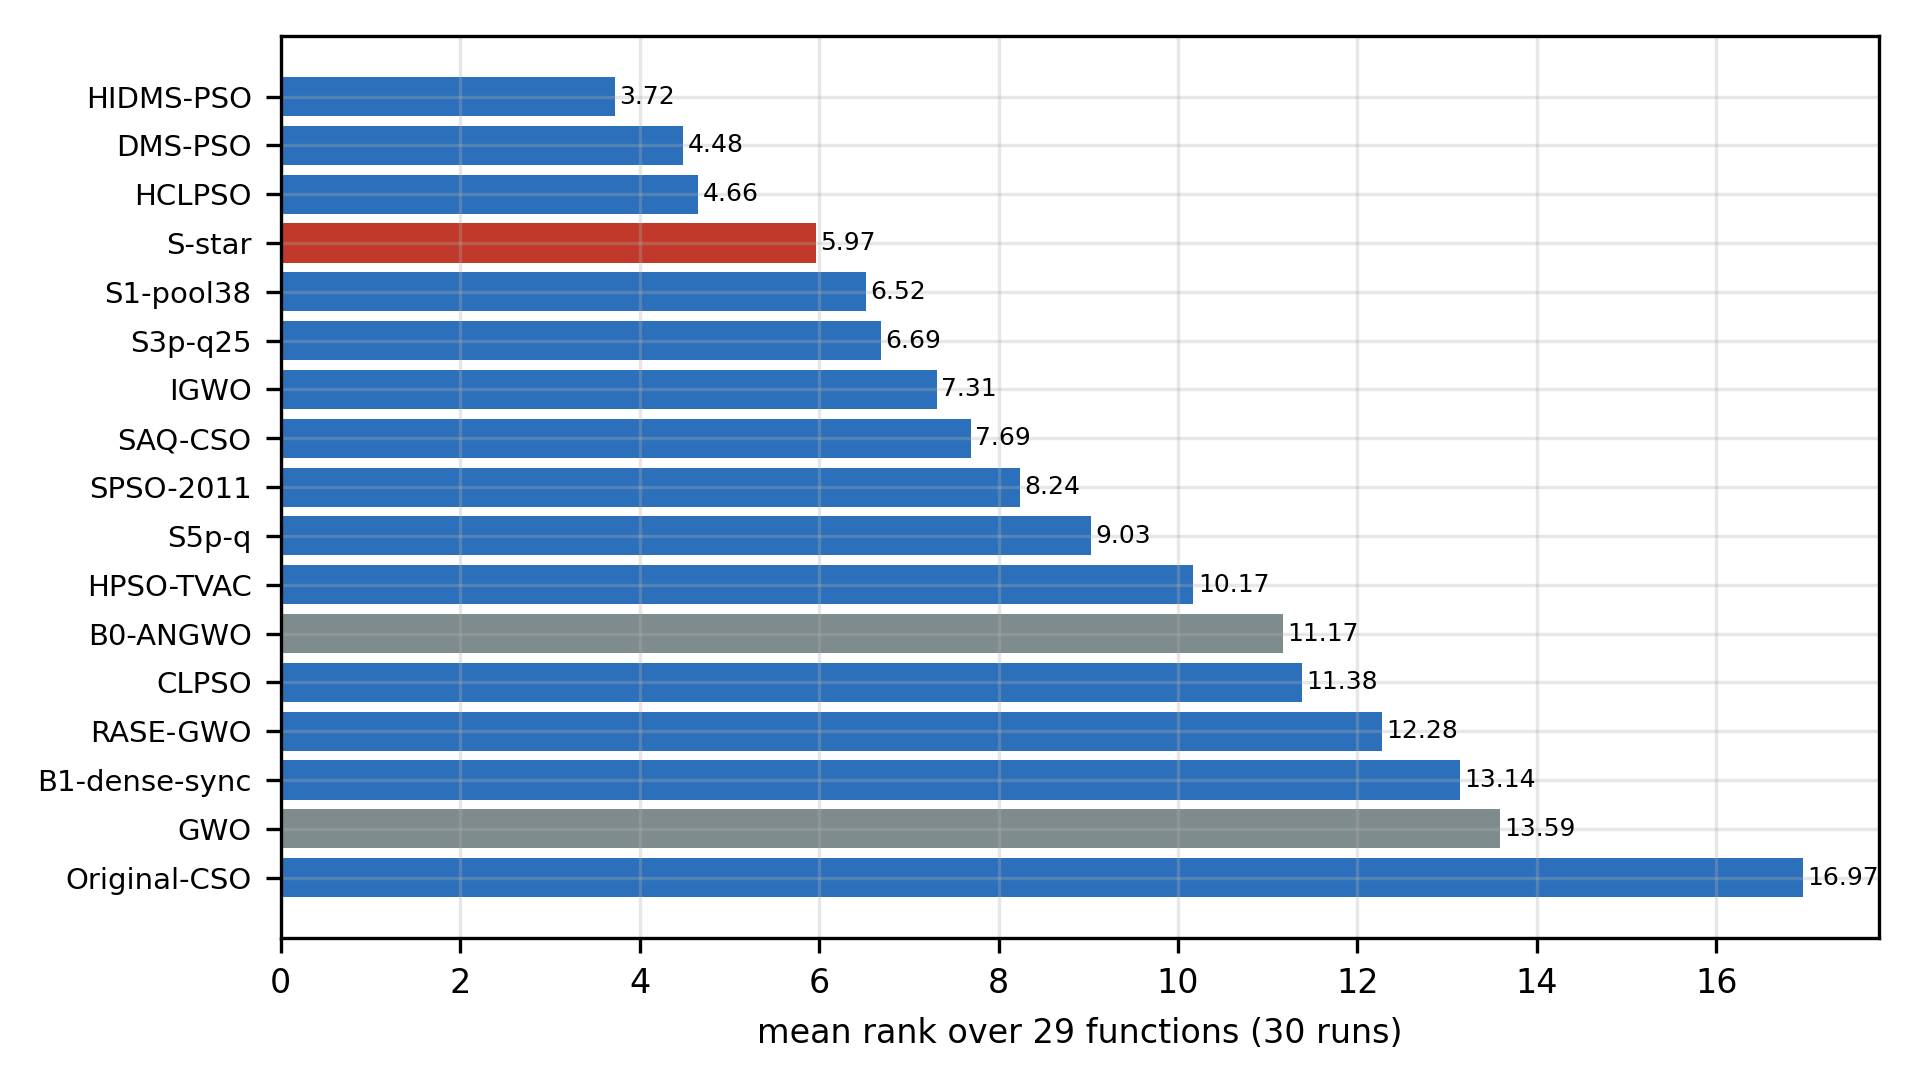
\includegraphics[width=\columnwidth]{figures/ranks.png}
\caption{Mean ranks over the 29 functions (30 runs each), CEC2017 $D=50$,
100{,}000 true evaluations. The frozen method is highlighted.}
\label{fig:ranks}
\end{figure}

\begin{figure*}[t]
\centering
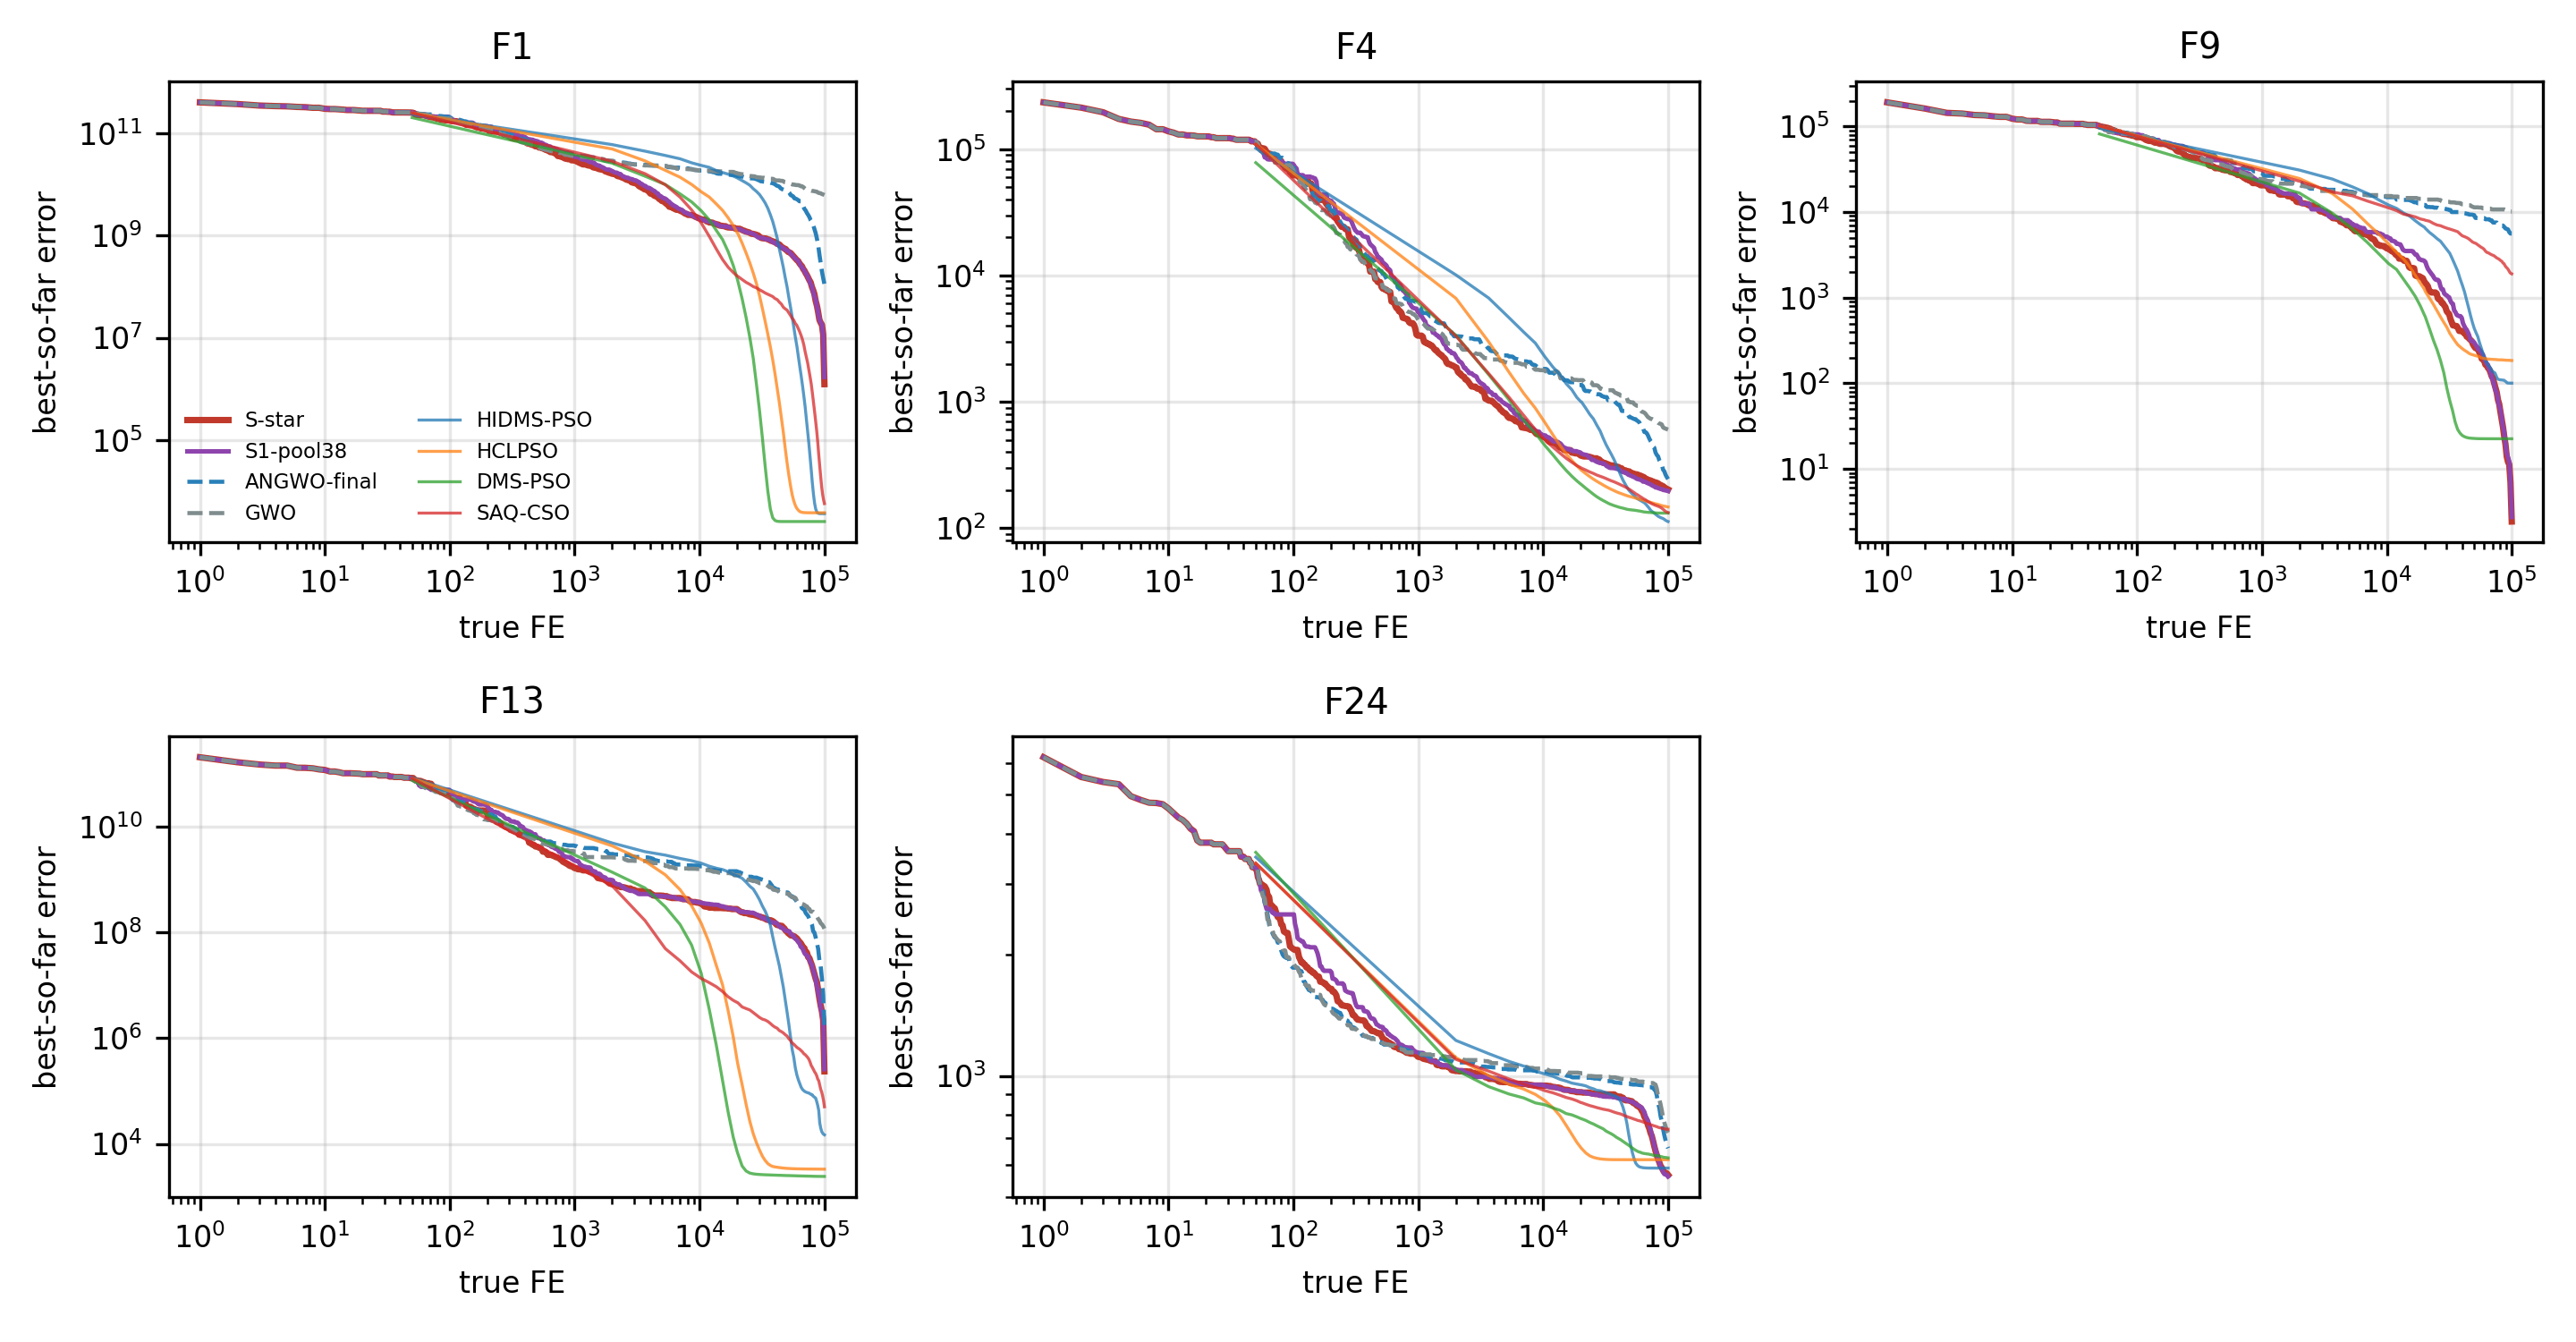
\includegraphics[width=\textwidth]{figures/convergence.png}
\caption{Median best-so-far error versus true evaluations on five
representative functions (F1, F4, F9, F13, F24). Thick red: frozen method;
purple: its K=50 variant; dashed grey: standard GWO; dashed blue: frozen
full-evaluation ANGWO; thin lines: audited strong baselines. All curves use
the same true-FE budget.}
\label{fig:conv}
\end{figure*}

\subsection{Early-budget behaviour}
At 10\% and 20\% of the budget the frozen method is already ahead of both
GWO (ratios 0.802 and 0.777; 25 and 26 function wins of 29) and the frozen
ANGWO (0.732 and 0.768; 27 wins), and the advantage grows to a 0.726 median
ratio against GWO at half budget. The finer evaluation granularity
($K=10$, hence 10{,}000 generations) is the mechanism behind the early
gains: the pack is updated in ten-evaluation increments instead of
fifty-evaluation generations, so the whole budget remains usable for
adaptive movement.

\subsection{Behaviour metrics}
Table~\ref{tab:behaviour} reports the probe-based behaviour metrics. The
frozen method recovers from stagnation episodes more often than both GWO
and the frozen ANGWO (0.823 versus 0.757 and 0.768), spends less of the
budget in long stagnation (0.813 versus 0.844 and 0.831), and roughly
doubles the fraction of its evaluations that convert into improvements
after being novel (useful novelty 0.0064 versus 0.0035 for GWO). The
improving-evaluation rate itself is \emph{lower} (0.0031 versus 0.0048 per
evaluation), which we read as fewer, better-placed discoveries rather than
more numerous ones --- the earlier-budget and better-recovery numbers show
where those discoveries land.

\begin{table}[t]
\centering
\small
\caption{Behaviour metrics on the formal tier (probe-instrumented
methods).}
\label{tab:behaviour}
\resizebox{\columnwidth}{!}{\begin{tabular}{lrrrrr}
\toprule
Method & Recovery prob. & Long-stag.\ share & Useful novelty & Nov.\ rate Q4 & Impr.\ rate Q4\\
\midrule
S-star & 0.823 & 0.813 & 0.00640 & 0.712 & 0.00308 \\
S1-pool38 & 0.816 & 0.812 & 0.00590 & 0.695 & 0.00266 \\
S3p-q25 & 0.808 & 0.821 & 0.00563 & 0.745 & 0.00272 \\
S5p-q & 0.780 & 0.835 & 0.00629 & 0.716 & 0.00264 \\
B0-ANGWO & 0.768 & 0.831 & 0.00578 & 0.690 & 0.00447 \\
GWO & 0.757 & 0.844 & 0.00347 & 0.588 & 0.00481 \\
\bottomrule
\end{tabular}}
\end{table}

\subsection{Scalability and resource tiers}
Two further tiers are reported in the repository. At $D=100$ (29 functions,
10 seeds, 100{,}000 evaluations) the frozen method again ranks first among
the five methods compared on the overlapping subset (mean rank 1.72 versus
S1-K50 2.00, RASE-GWO 2.33, dense-sync 3.52 and I-GWO 3.67), with a
$0.703$ median ratio and $10$ wins against $2$ losses (Holm $+5/-1$) against
I-GWO on its 12-function subset, at a cost of 11.97\,s per run. Under a
severely constrained budget (20{,}000 evaluations, 29 functions, 10 seeds)
the method ranks first as well (1.97 versus 2.31 for S1-K50 and 3.83 for
GWO), winning 24 of 29 functions against GWO (ratio 0.721) and 24/29
against the frozen ANGWO (0.807). The sparse framework therefore scales
with dimension and with smaller budgets rather than relying on the
100{,}000-evaluation regime.


\section{Application: 3D UAV Delivery Path Planning}
\label{sec:uav}
The sparse-evaluation framework is applied to a three-dimensional UAV delivery
scenario built on five real Copernicus GLO-90 digital-elevation tiles (ridge,
peaks, mountain, hills and plateau). Each instance contains 20 delivery
stations with hard time windows, three cylindrical threat zones and three
intermediate control points per leg, i.e.\ a 209-dimensional mixed
route-and-trajectory search space; this is a normalized simulation derived from
real terrain data, not a flight test. All algorithms use $N=50$, 30{,}000 true
fitness evaluations (initialization included), identical initial populations
per (map, seed) and 30 seeds (101--130). The comparison set is GWO, I-GWO,
HAGWO (2026), PSO and CLPSO; 900/900 runs completed with zero failures.

\begin{table}[t]
\centering
\caption{3D UAV application (150 runs per method). Feas.: routes found within
30{,}000 evaluations; RMST: restricted mean time to first feasibility under a
30{,}000-evaluation censoring horizon (lower is better); medians in FE.}
\label{tab:uav}
\begin{tabular}{lcccc}
\toprule
Method & Feas.\ (\%) & RMST & Med.\ first feas. & Med.\ cost \\
\midrule
VAST-GWO & \textbf{100.0} & \textbf{7062} & 6314 & 667.4 \\
GWO      & 94.0 & 10936 & 8920 & 699.8 \\
I-GWO    & 97.3 & 12270 & 11152 & 724.7 \\
HAGWO    & 97.3 & 8133 & 7432 & 663.4 \\
PSO      & 95.3 & 8138 & 5357 & 766.4 \\
CLPSO    & 61.3 & 24427 & 21330 & 1015.4 \\
\bottomrule
\end{tabular}
\end{table}

\begin{figure}[t]
\centering
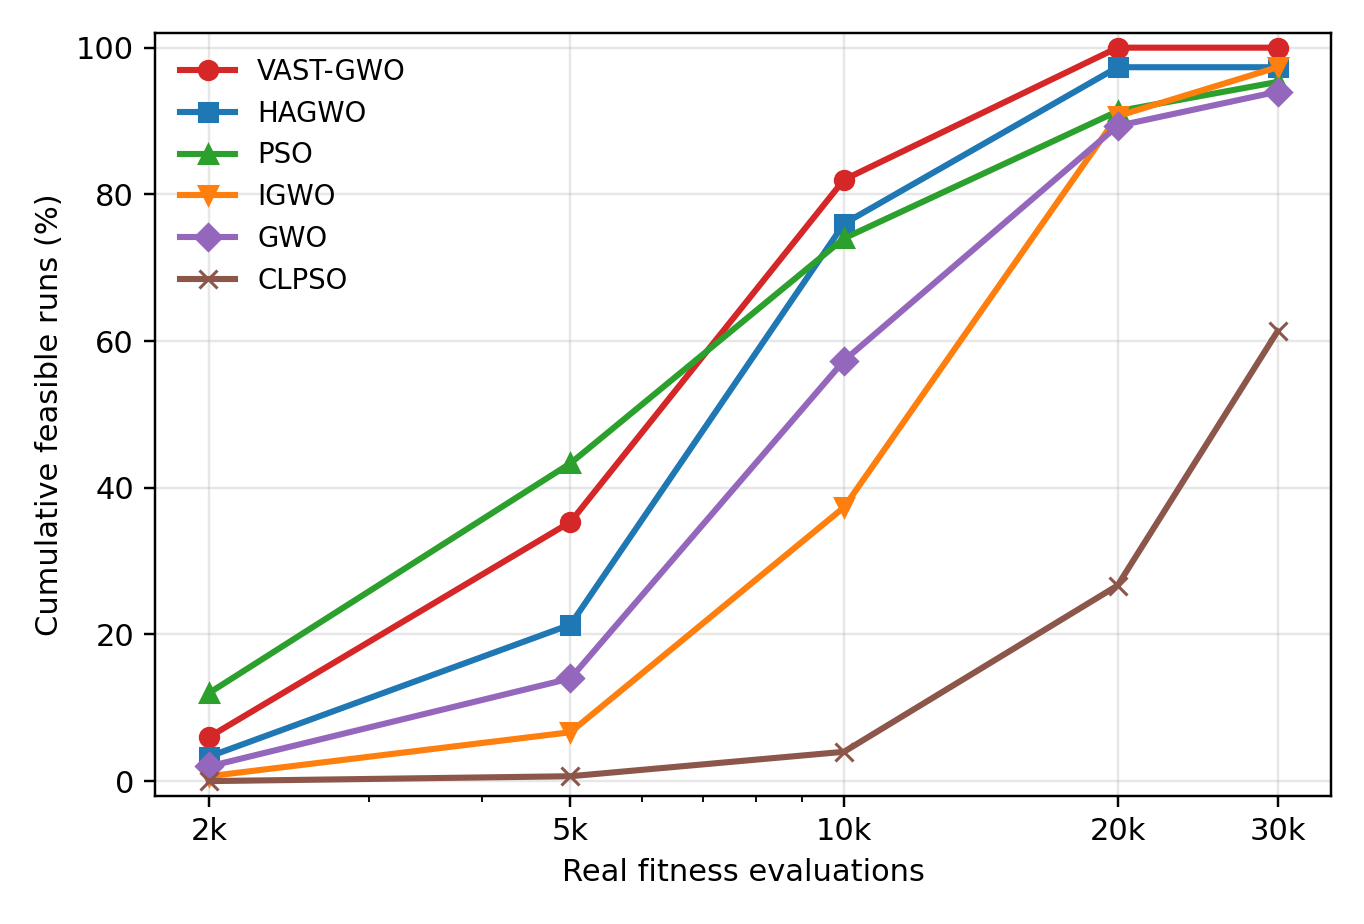
\includegraphics[width=\columnwidth]{figures/uav_feasibility_curve.png}
\caption{Cumulative feasible runs versus real fitness evaluations
(benchmark-v1, six methods, 150 runs each). The checkpoints at 2k--20k are
early observations within the single 30k protocol, not independent
short-budget runs.}
\label{fig:uavfeas}
\end{figure}

\begin{figure}[t]
\centering
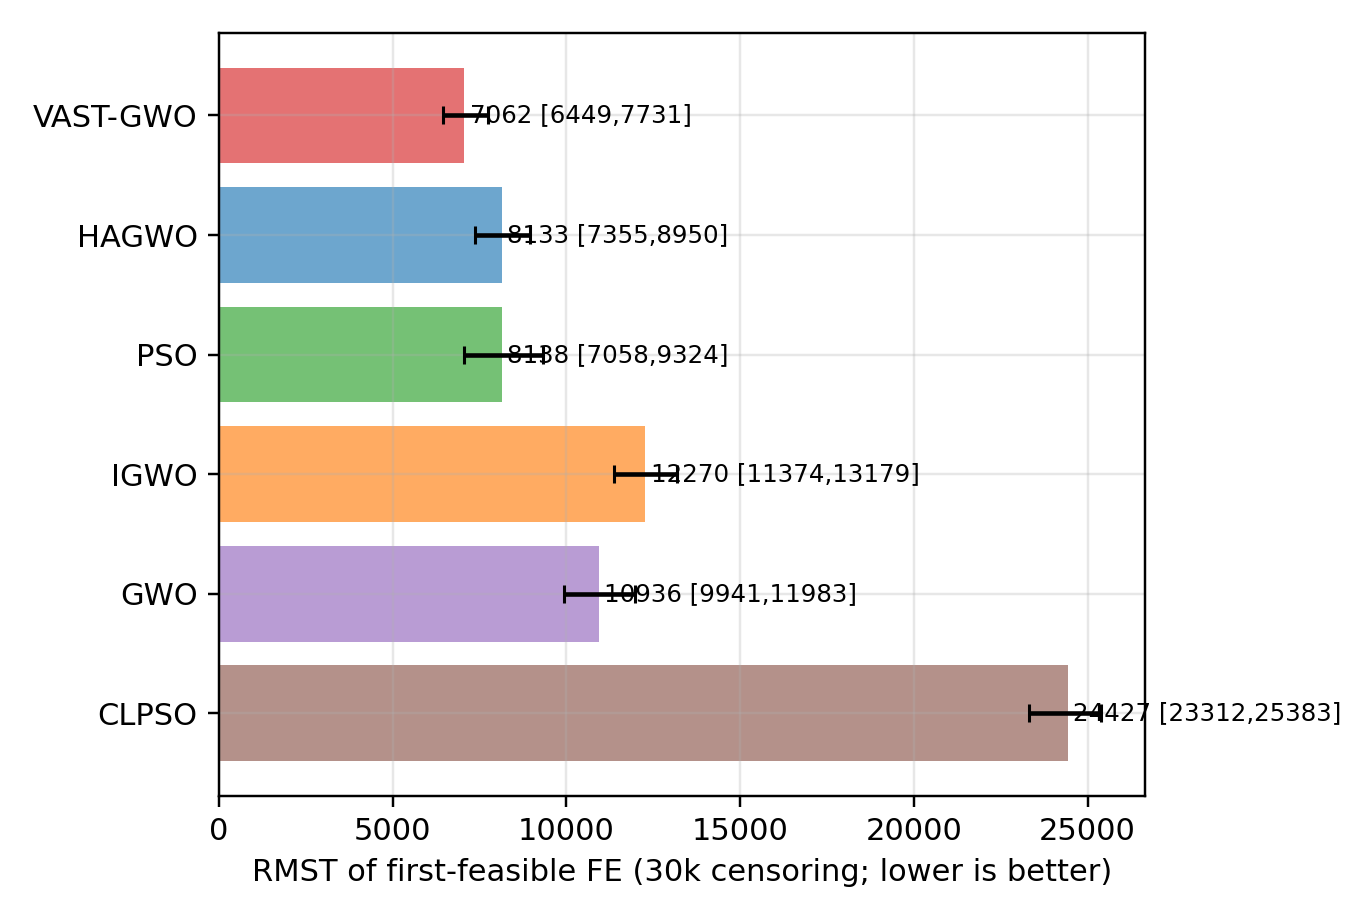
\includegraphics[width=\columnwidth]{figures/uav_rmst_bar.png}
\caption{Restricted mean time to first feasible route (30k censoring,
bootstrap 95\% CI). All runs, including those that never reach feasibility,
enter the statistic.}
\label{fig:uavrmst}
\end{figure}

\method{} is the only method that finds a feasible route in every one of the
150 runs (100\% versus 97.3\% for I-GWO and HAGWO, 95.3\% for PSO, 94.0\% for
GWO and 61.3\% for CLPSO; Table~\ref{tab:uav}). Under the censoring horizon its
RMST is the smallest ($7062$, $95\%$ CI $6449$--$7731$), i.e.\ it also reaches
feasibility fastest on average once failed runs are accounted for
(Figure~\ref{fig:uavrmst}); the advantage grows in the mid-to-late budget
(82.0\% versus 76.0\%/74.0\% at 10{,}000 evaluations; 100\% versus
97.3\%/95.3\% at 20{,}000; Figure~\ref{fig:uavfeas}). Paired tests over the
150 map--seed pairs (Holm across the five baselines) give significantly better
final cost against every baseline (median ratios $0.631$--$0.967$, Holm
$p\le 0.046$) and significantly earlier censored time-to-feasibility against
GWO, I-GWO, HAGWO and CLPSO ($p\le 0.0072$).

Two non-supported comparisons are reported explicitly. PSO discovers feasible
routes earlier in the first 5{,}000 evaluations and its paired
time-to-feasibility difference is not significant ($p=0.598$ on the
checkpoint-ordered test), but its final routes are worse (median cost $766.4$
versus $667.4$). HAGWO's marginal median cost ($663.4$) is slightly below that
of \method{} ($667.4$) because it conditions on its own successful runs; on
the 146 pairs where both succeed, \method{} is significantly better (median
ratio $0.967$, rank-biserial $0.19$, Holm $p=0.0458$) and it is more reliable.
\section{Ablation and Mechanism Study}
\label{sec:ablation}
The design space was explored on an eight-function development set
($D=30$, 30{,}000 evaluations, seeds 3001--3010 plus an unseen confirmation
set 3011--3020) under pre-registered gates; every rejected alternative is
retained. Unless stated, ratios compare paired runs on identical
(function, seed) pairs and a ratio below one favours the variant.

\subsection{Pool composition and evaluation density}
Enlarging the multi-region share beyond the pool proportion hurts
($q_E=0.50$: 1.06; $q_E=0.75$: 1.67 versus uniform selection); shrinking it
does not help (pinned 25\% quota: 1.02--1.09 across two seed sets). The
uniform policy over the pool is therefore not a compromise but the optimum
of the tested family. For the evaluation density, $K=10$ beat $K=50$
consistently on both development seed sets (0.970 with 6/8 wins, and 0.955
with 6/8 wins, $p=0.053$), which motivated the frozen $K=10$; the formal
tier confirms the choice (S-star 0.525 versus S1-pool38 0.541 against GWO,
with the earlier-budget advantage).

\subsection{Screening rules are falsified}
Directed screening (nearest-incumbent refinement slots plus
credit-weighted multi-region centres) is worse than uniform random
selection of the same pool (median ratio 1.39); history-informed assignment
inside stratified slots is worse still (1.53). The mechanism is visible in
the first-generation composition audit: uniform selection evaluates
$[G_1,G_2,E]=[24,10,16]$ candidates on average, identical in expectation to
the stratified allocation, so the loss cannot come from the quota --- it
comes from starving the pack's own leader-aggregation moves of evaluations,
after which the verified population stops advancing.

\subsection{Quota policies and Q-learning}
Fixed quotas away from the pool proportion and randomly perturbed quotas
both degrade performance (random quota: 1/7 function wins, $p<10^{-3}$).
Three Q-learning schedulers were tested with the pre-registered 6-state
(progress $\times$ stagnation) by 3-action (exploration share
$\{0.25,0.50,0.75\}$) design and per-500-FE reward windows combining the
normalized global-best improvement with a small verified-record term:
(i) zero-initialized table, (ii) tuned $\alpha=0.3$, $\gamma=0.95$, fast
$\varepsilon$-decay, and (iii) prior-initialized table. Their ratios against
the best fixed quota at 10 development seeds were 0.988, 1.024 and 1.130
(win rates 3/8, 2/8, 4/8); in the formal tier the Q variant (S5p-q) ranks
9.03 against the fixed-quota variant's 6.69. The schedulers do beat
\emph{random} quota perturbation (0.75--0.87), but never the best constant;
the prior-initialized variant degenerates to 93\% single-action play. We
therefore conclude that the lightweight Q scheduler has no independent
benefit in this setting, and the frozen method contains no RL component ---
an outcome consistent with earlier findings that the screening term, not
the scheduler, carries such frameworks.

\subsection{Post-freeze enhancement probes}
Three additional single-change enhancements were screened after the frozen
batch: (i) stagnation-triggered radius inflation of the shell candidates
($\times3$): 1.20, rejected; (ii) reuse of \emph{verified success
directions} --- 25\% of the refinement moves are extended by half a median
successful step along a recorded improving displacement: 0.934 (5/8), a
passing but small effect; (iii) coordinate-subset perturbation of the
incumbent shells (20\% of dimensions): error-neutral (0.991) but with a
large stagnation-axis gain (recovery 0.887 versus 0.815, long-stagnation
share 0.785 versus 0.852, useful novelty $+28\%$). The combination and a
fresh-seed confirmation are reported in the accompanying repository; they
are deliberately kept outside the frozen claim.

\section{Discussion}
\label{sec:discussion}
\subsection{Dual-axis verdict}
The pre-registered gates separate two claims. \emph{Exploration efficiency
(A): supported.} At 20\% of the budget the frozen method is 23\% better
than the frozen ANGWO on median (0.768, 26/29 wins), 29\% better on the
simple-multimodal family (0.714), and its useful-novelty rate is 11\%
higher (0.00640 versus 0.00578). \emph{Stagnation recovery (B): partially
supported.} The recovery probability rises by 5.6 percentage points
(0.823 versus 0.768; gate $+0.05$ passed) and the long-stagnation share
falls by 1.8 points (0.813 versus 0.831; the pre-registered $0.03$ gate is
\emph{not} passed). We therefore claim axis A and report axis B as
partially supported, with the failed half stated explicitly.

\subsection{Why the simple policy wins}
Three independent comparisons point the same way: uniform random selection
over a dual-route pool beats geometry-directed screening (1.39), pinned
stratified allocation (1.02--1.09), random quota perturbation (1/7 wins)
and learned quota scheduling (0.99--1.13 against the best constant). The
interpretation is structural, not statistical: in a leader-driven method,
the dominant information channel is that each wolf's own move receives
real evaluations; screening or scheduling that concentrates evaluation
slots away from this channel starves the population, while the dual-route
pool itself continuously injects verified multi-region candidates. This is
consistent with the earlier observation that evaluations near the incumbent
convert an order of magnitude more often than far-away ones.

\subsection{Limitations}
(i) The method remains behind the three strongest multi-swarm PSO variants
(median ratios 1.04--1.23; losses on F1 by three orders of magnitude on the
ill-conditioned unimodal function, and on F6/F19/F30); it ties rather than
beats I-GWO and SAQ-CSO. (ii) The frozen $K=10$ costs about
$1.6\times$ GWO's wall-clock (5.93\,s versus 3.63\,s on four workers) and
$2.6\times$ I-GWO's. (iii) The Q-learning component --- a headline of the
investigated direction --- is reported as \emph{not beneficial}; we keep it
as a fully documented negative result rather than claiming RL. (iv) The
study is CEC2017-only; the $D=100$ tier and a 20{,}000-evaluation resource
tier are reported separately in the repository, and no engineering
application is included. (v) The post-freeze enhancements (success-direction
reuse, coordinate-subset shells) show promise on single axes but are not
part of the frozen claim.

\section{Conclusion}
This paper studied what a grey wolf pack should spend its scarce true
evaluations on. A minimal dual-route sparse framework --- refinement
candidates near the incumbent plus verified multi-region candidates from an
elite archive, with $K=10$ uniformly sampled evaluations per generation and
a strict verified-state discipline --- improves standard GWO by a median
factor of 0.525 with 24 Holm-significant wins and no significant losses,
overtakes the frozen full-evaluation ANGWO and the historical sparse
RASE-GWO, and reaches statistical parity with author-faithful I-GWO and
with sparse adaptive-quota CSO while remaining behind the strongest
multi-swarm PSO variants. A complete pre-registered ablation shows that
directed screening, stratified allocation, fixed quota deviation, random
quota perturbation and three Q-learning schedulers all fail to beat the
simple policy; the exploration-efficiency axis is supported, the stagnation
recovery axis is partially supported, and the RL component is reported as
an honest negative result.\bibliographystyle{IEEEtran}
\bibliography{references}

\end{document}







